\chapter{Player Strategies}
In this section the players' strategies are briefly described. For the whole document there are some definitions to be explained:
\begin{itemize}
	\item \textbf{Make move:} Placing a given piece on a cell of the board
	\item \textbf{Select piece:} Choosing a piece for the opponent
	\item \textbf{Perform action:} Making move first, then choosing a piece
\end{itemize}
\section{Random Player}
The most trivial player. Performs his actions randomly with only one restriction: He can't make a move on a taken cell and he can't select a piece that has already been chosen.
\section{Novice Player}
Acts the same way as Random Player does, bit in cases, where he can make a move in order to win, he will make this move. The same applies to the chosen a piece, as he won't select a piece for his opponent that might make the opponent win with only one move. If there are no such pieces left, he chooses a piece randomly.
\section{Monte Carlo Player}
Every time this player has to perform an action, he simulates hundreds of games for each possible action he can perform. He chooses the action which has led to the most wins during the simulations. Usually, Monte Carlo simulations are totally random, but we used the Novice Player for the simulations instead. To speed the simulations up, they are performed parallely.
\section{MinMax-D Player}
The MinMax-D Player looks $D$ actions into future. One action means that only one player selects a piece and makes a move, but not both of them. So for $D=3$ the player simulates all possible actions he can perform, all possible counteractions to these actions and all possible counteractions to the counteractions. We use $\alpha$-$\beta$-pruning in order to reduce the number of nodes being evaluated.

We use the Monte Carlo strategy before the seventh piece is set on the board.

During the search, if the MinMax player comes upon a state, where the game is either won, lost or tied it's easy to evaluate such a state. But when a leaf in the search tree is a intermediate state, it has to be evaluated otherwise.
\subsection{Evaluation functions}
In order to test the further evaluation functions we used a trivial function that always return 0 regardless of the state of the board. A MinMax-D Player with such an evaluation function behaves the like a Novice Player with $D$ actions foresight.
\subsubsection*{Almost Completed Attributes}
This evaluation function determines how many attributes there are which are almost completed. For an almost completed attribute there must be a row with three pieces which have this attribute in common. Consider figure \ref{fig:almostCompletedRows}. Here, there are three almost completed attributes. The pieces in the row share the attribute \emph{BIG} and \emph{SOLID}, the pieces in the column are \emph{BLUE} and the diagonal consits of \emph{CIRCLULAR} pieces.

The evaluation function counts all almost completed attributes and returns this number.
\begin{figure}[h]
  \centering
  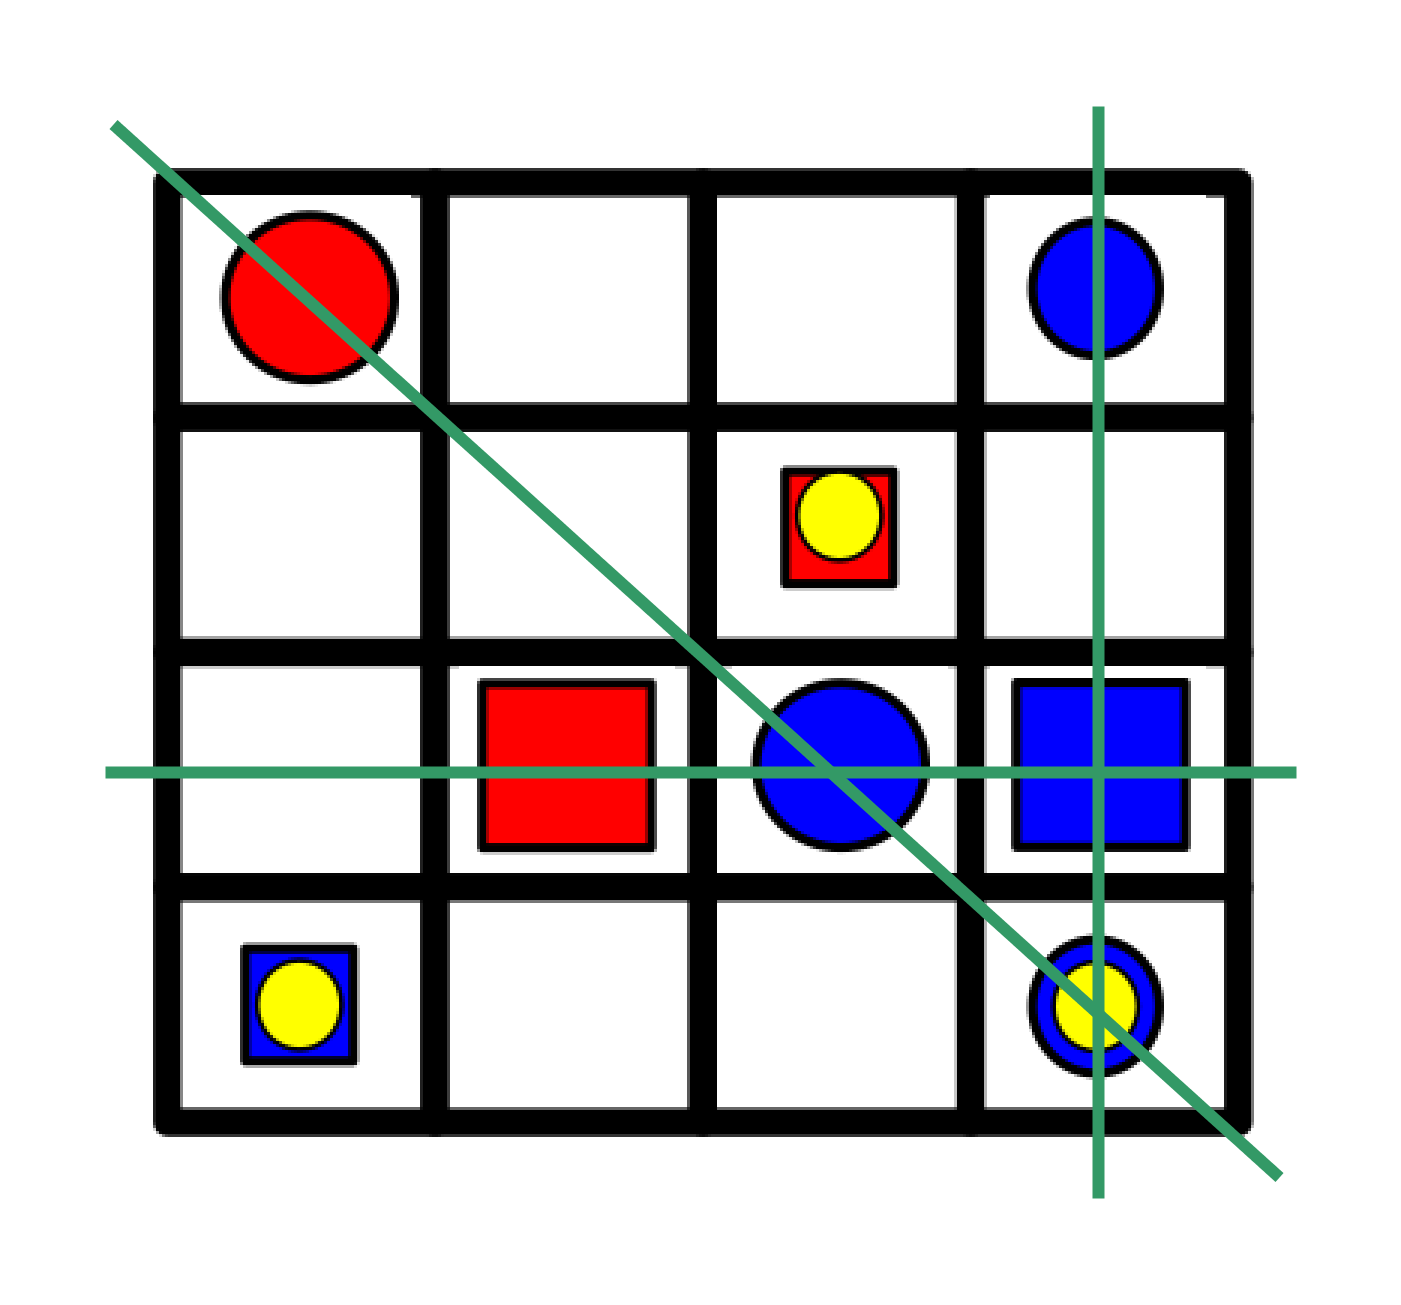
\includegraphics[width=0.3\textwidth]{images/almostCompletedRows}
  \caption{A board with four almost completed attributes}
  \label{fig:almostCompletedRows}
\end{figure}
\subsubsection*{Completing Pieces: Absolute}
In the previous evaluation function the remaining pieces aren't taken into account. Now, we want to correct this. The reason why this is important is shown in figure \ref{fig:completingPiecesAbsoluteB}. Here, there are two almost completed attributes (\emph{BIG}) but no pieces left to complete these attributes. Therefore, these attributes don't give any advantage to the player.
\begin{figure}[h]
  \centering
  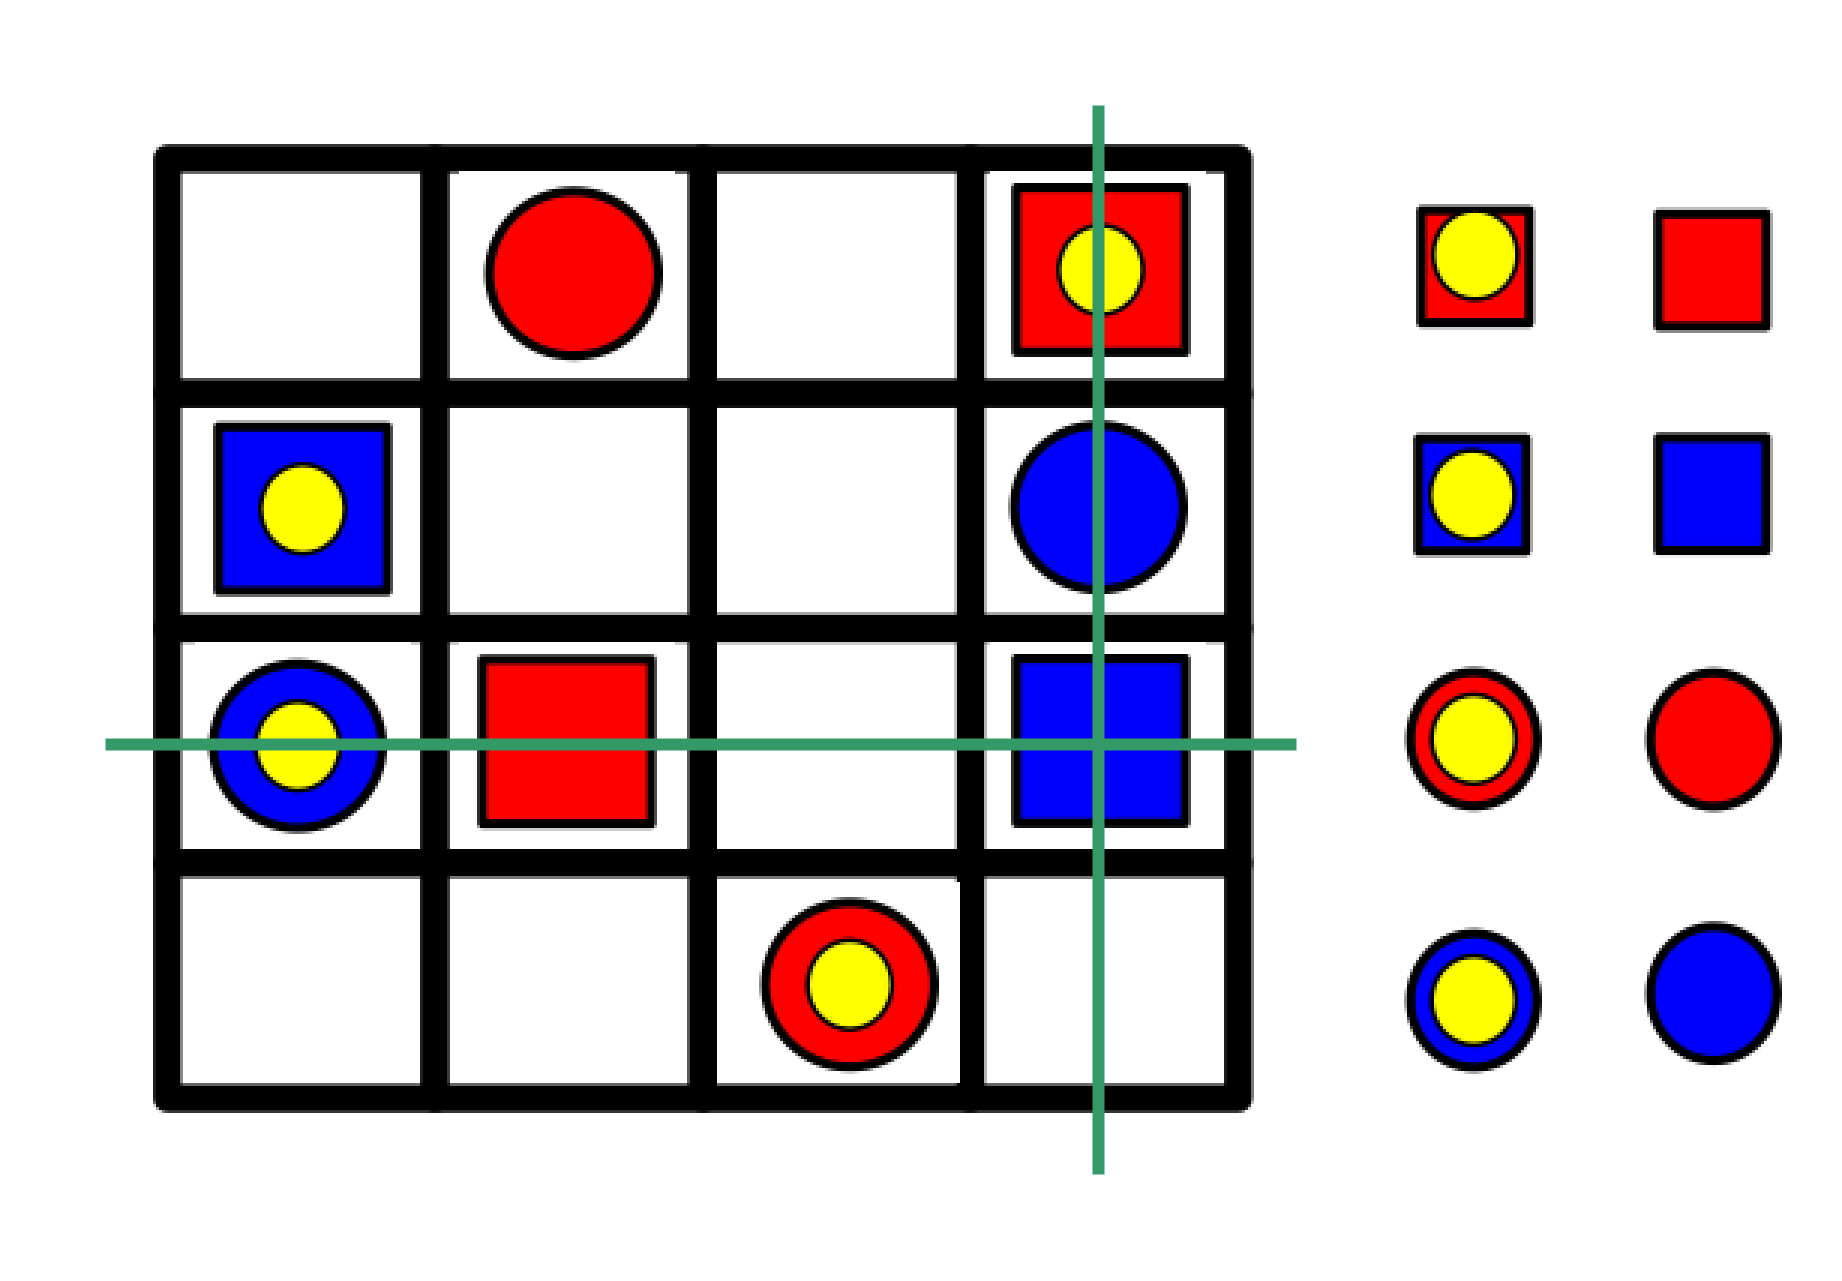
\includegraphics[width=0.5\textwidth]{images/completingPiecesAbsoluteB}
  \caption{A board with two almost completed attributes but no pieces to complete these attributes}
  \label{fig:completingPiecesAbsoluteB}
\end{figure}

Similarly to the previous evaluation function we determine which attributes are almost completed. But now we also iterate through the remaining pieces and count the pieces which can complete one or more of the attributes. If a piece completes more than one attribute, it is counted more than once. The figure \ref{fig:completingPiecesAbsoluteA} show a board with 15 completing pieces. There are 4 pieces to complete the attribute \emph{BIG}, 4 pieces to complete \emph{SOLID}, 3 pieces to complete \emph{BLUE} and 4 pieces for \emph{CIRCULAR}.
\begin{figure}[h]
  \centering
  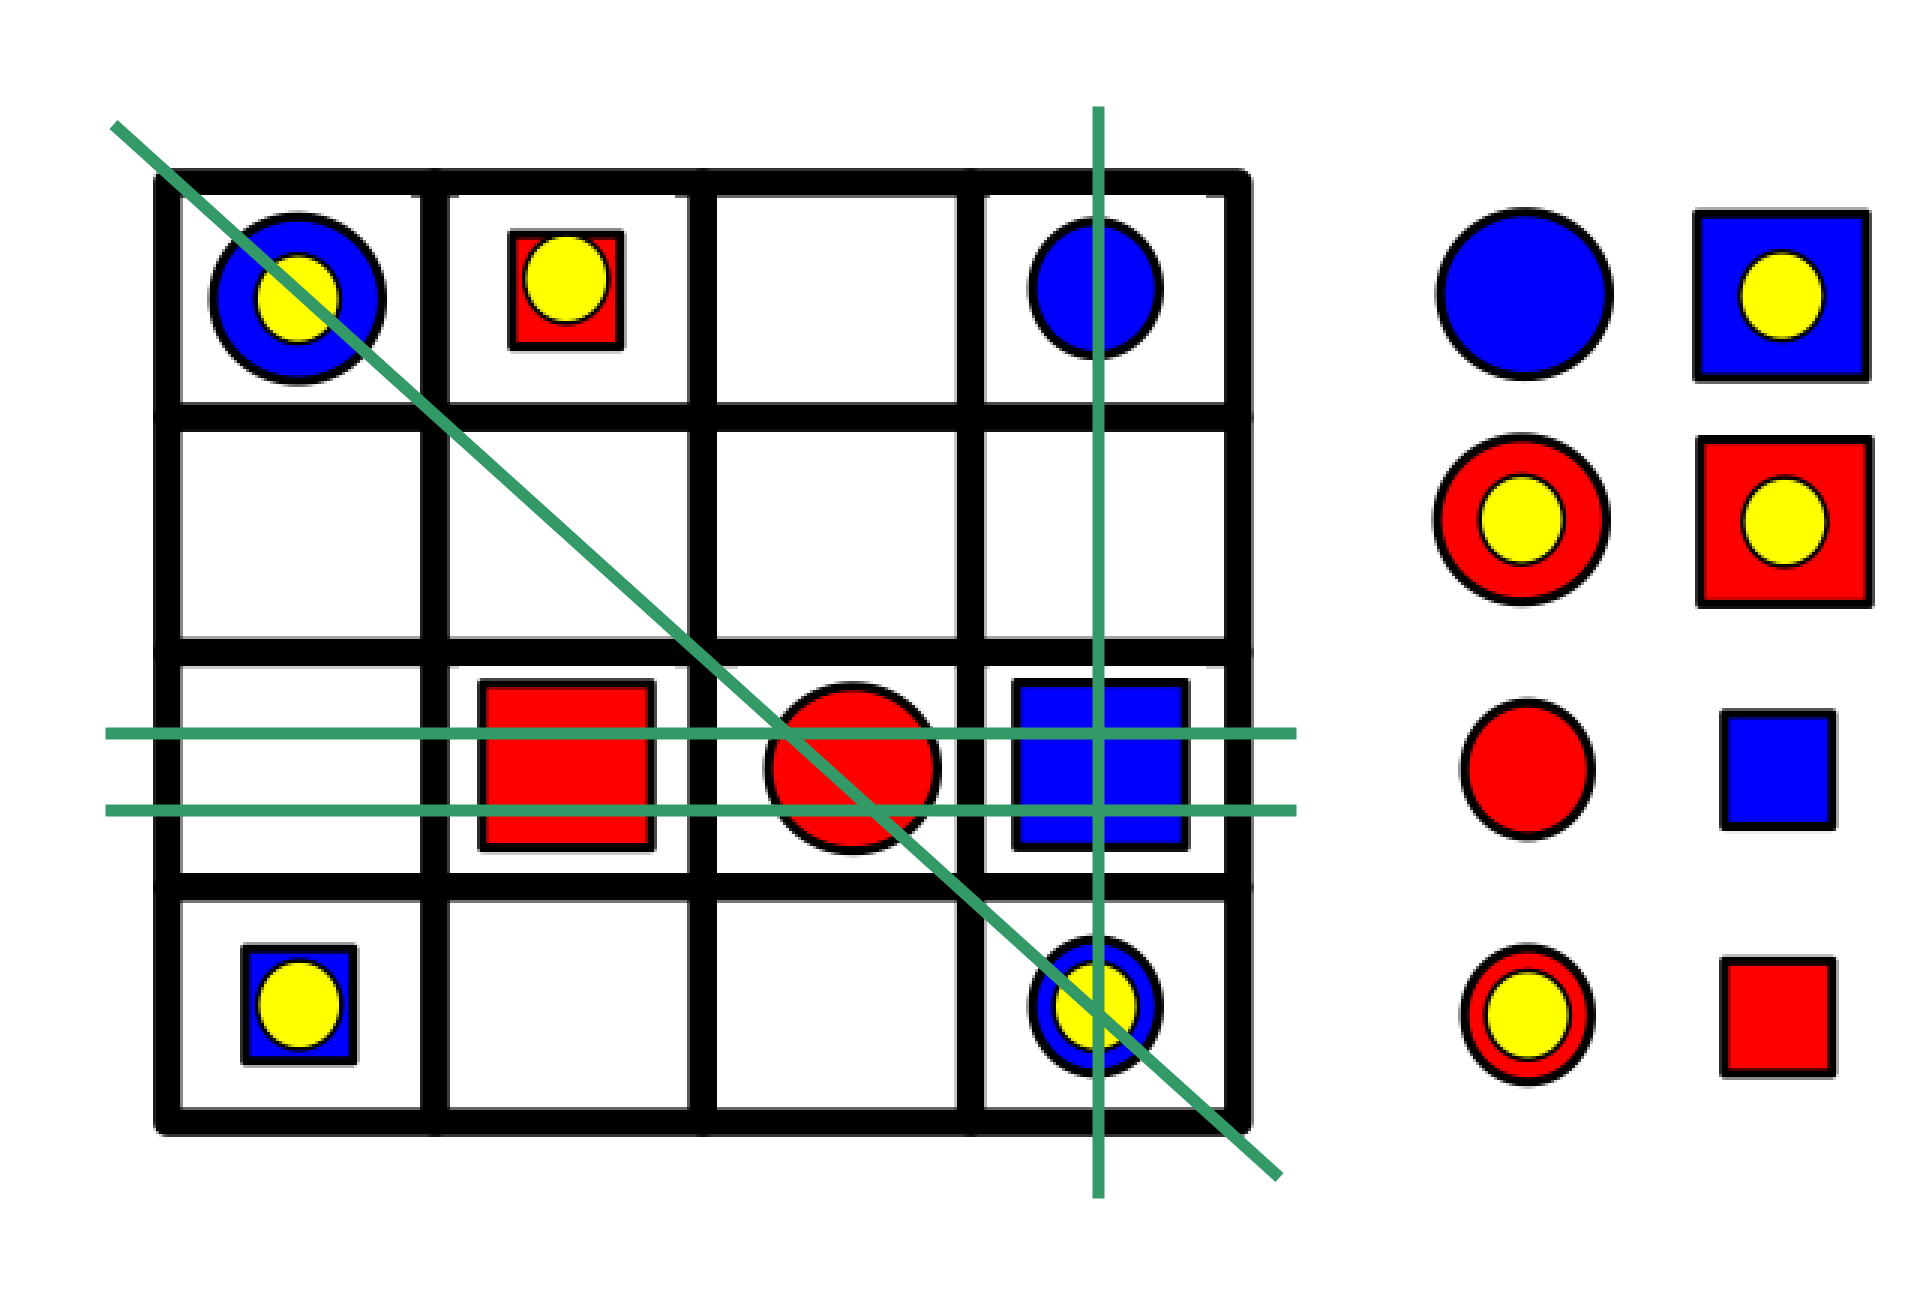
\includegraphics[width=0.5\textwidth]{images/completingPiecesAbsoluteA}
  \caption{A board with three almost completed attributes and several pieces which complete an attribute}
  \label{fig:completingPiecesAbsoluteA}
\end{figure}
\subsubsection*{Completing Pieces: Relative}
In the previous evaluation function the pieces which complete an attribute are taken into account, but the pieces which don't complete anything are left out. It is interesting to see if these pieces would improve the estimation of a board state.

Therefore, we don't only determine the number of completing pieces but also set this number in relation to the amount of remaining pieces. The value $h$ returned by the evaluation function is shown in equation \ref{equ:relativeEvaluationEquation}. $C$ is a constant stretching factor.
\begin{equation}
	\label{equ:relativeEvaluationEquation}
	h=\frac{\#~completing~pieces}{\#~remaining~pieces}*C
\end{equation}

Figure \ref{fig:relativeComparison} illustrates the implications that the equation \ref{equ:relativeEvaluationEquation} has. The evaluation function returns $h = 0.27$ for the left and $h = 0.5$ for the right board. That means that the right board is considered more desirable. The reason for this is, that the evaluation happens at a moment when the opponent has made a move. In the next step the opponent selects a piece for us. The right state in figure \ref{fig:relativeComparison} has less pieces that can't complete a row, which is good for us. 
\begin{figure}[h]
  \hspace*{-7mm}
  \begin{minipage}[b]{0.5\linewidth}
    \centering
    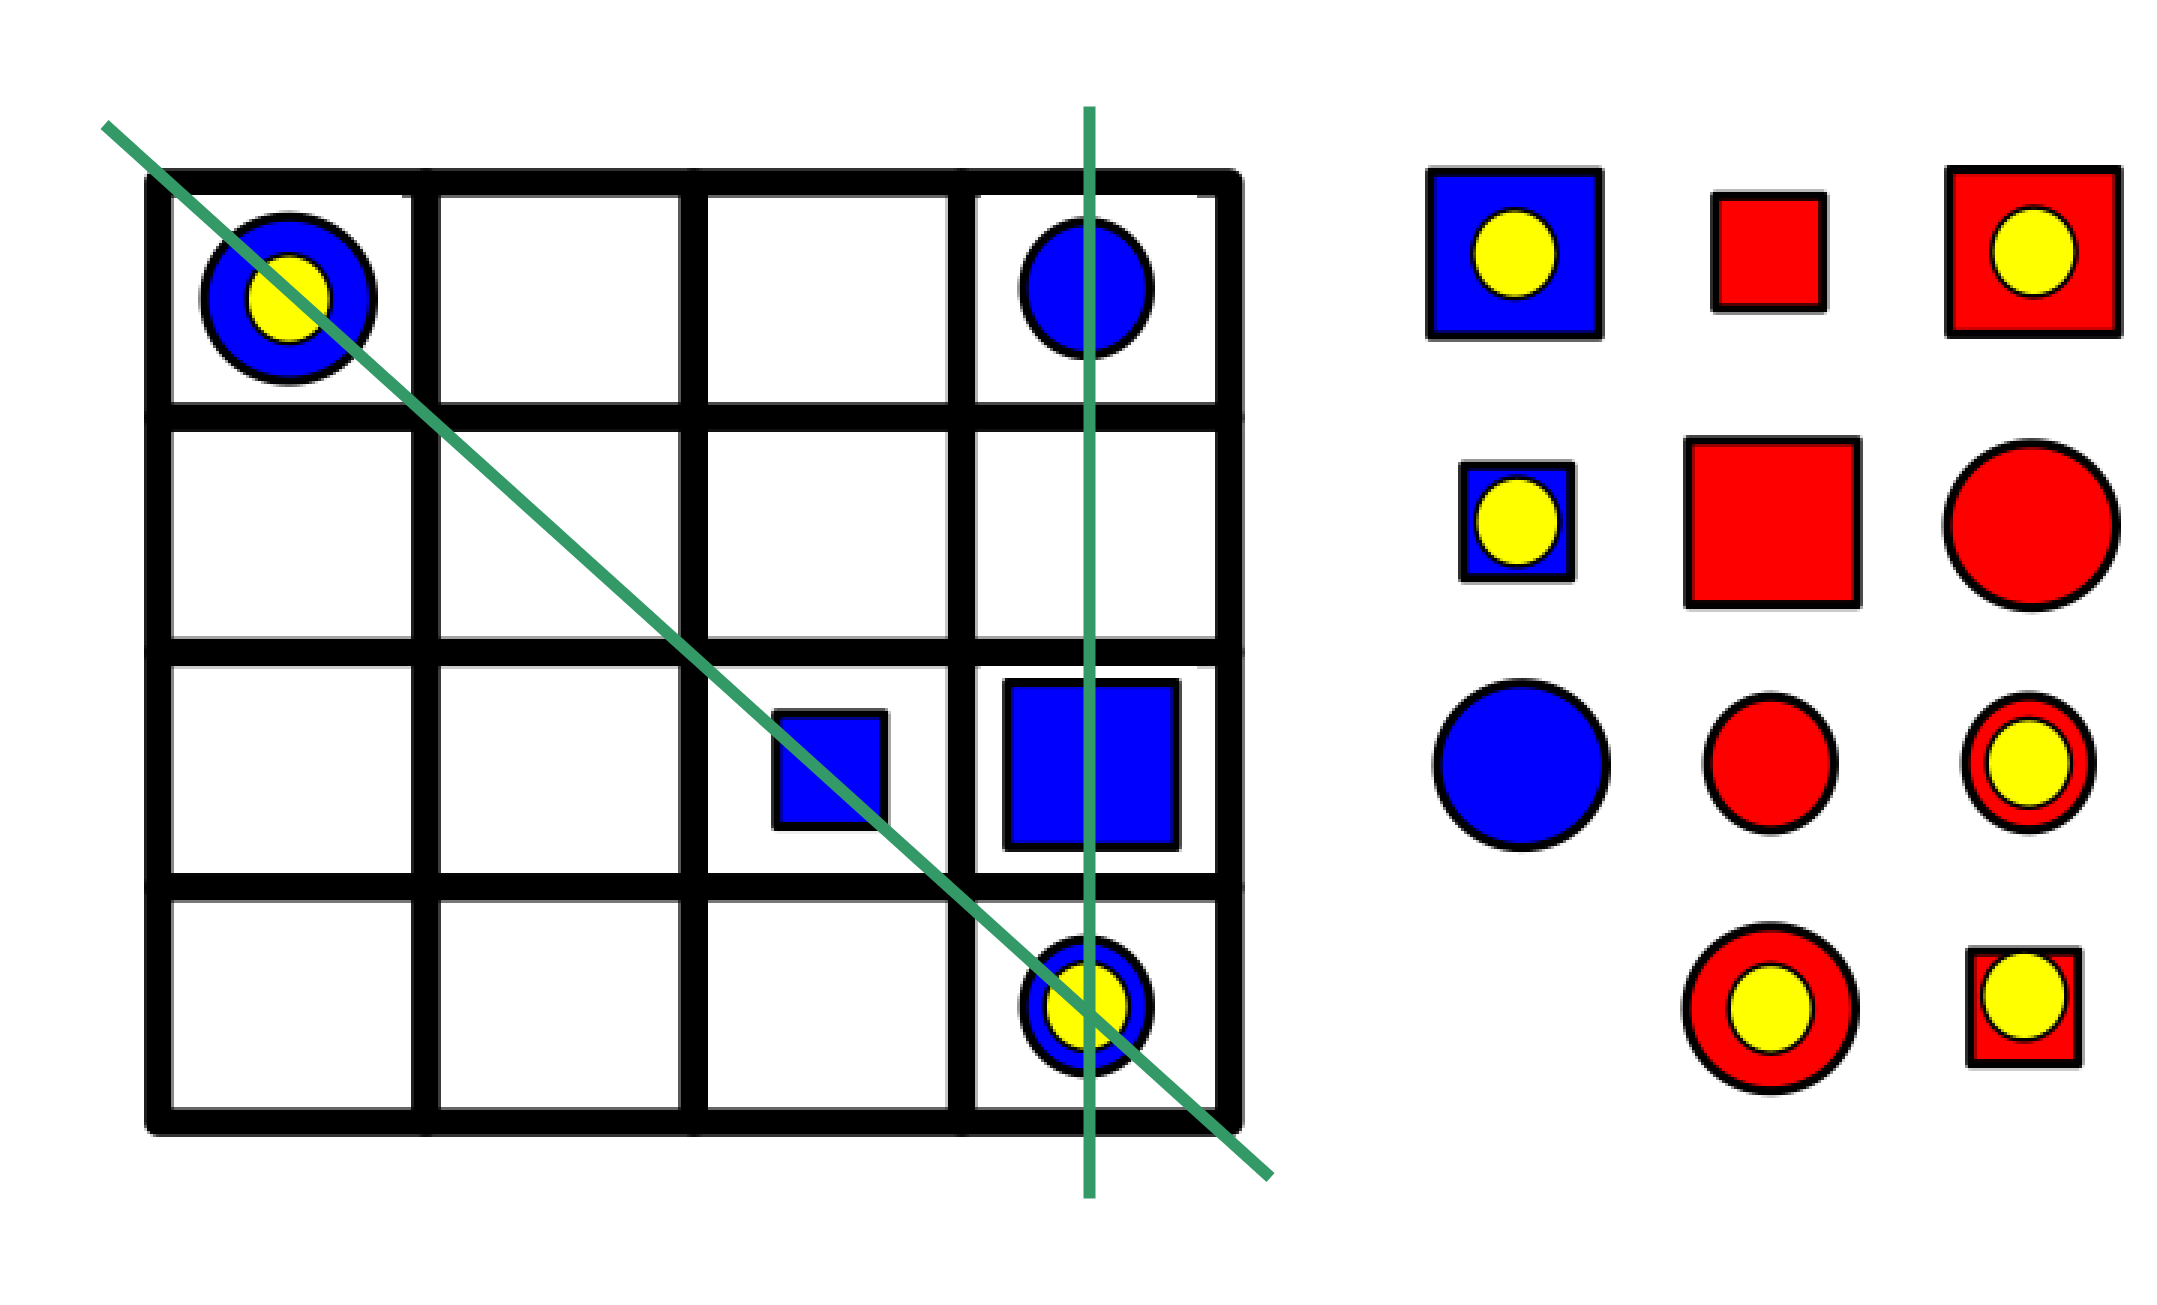
\includegraphics[height=0.2\textheight]{images/completingPiecesRelativeC}
  \end{minipage}
  \hspace{10mm}
  \begin{minipage}[b]{0.5\linewidth}
    \centering
    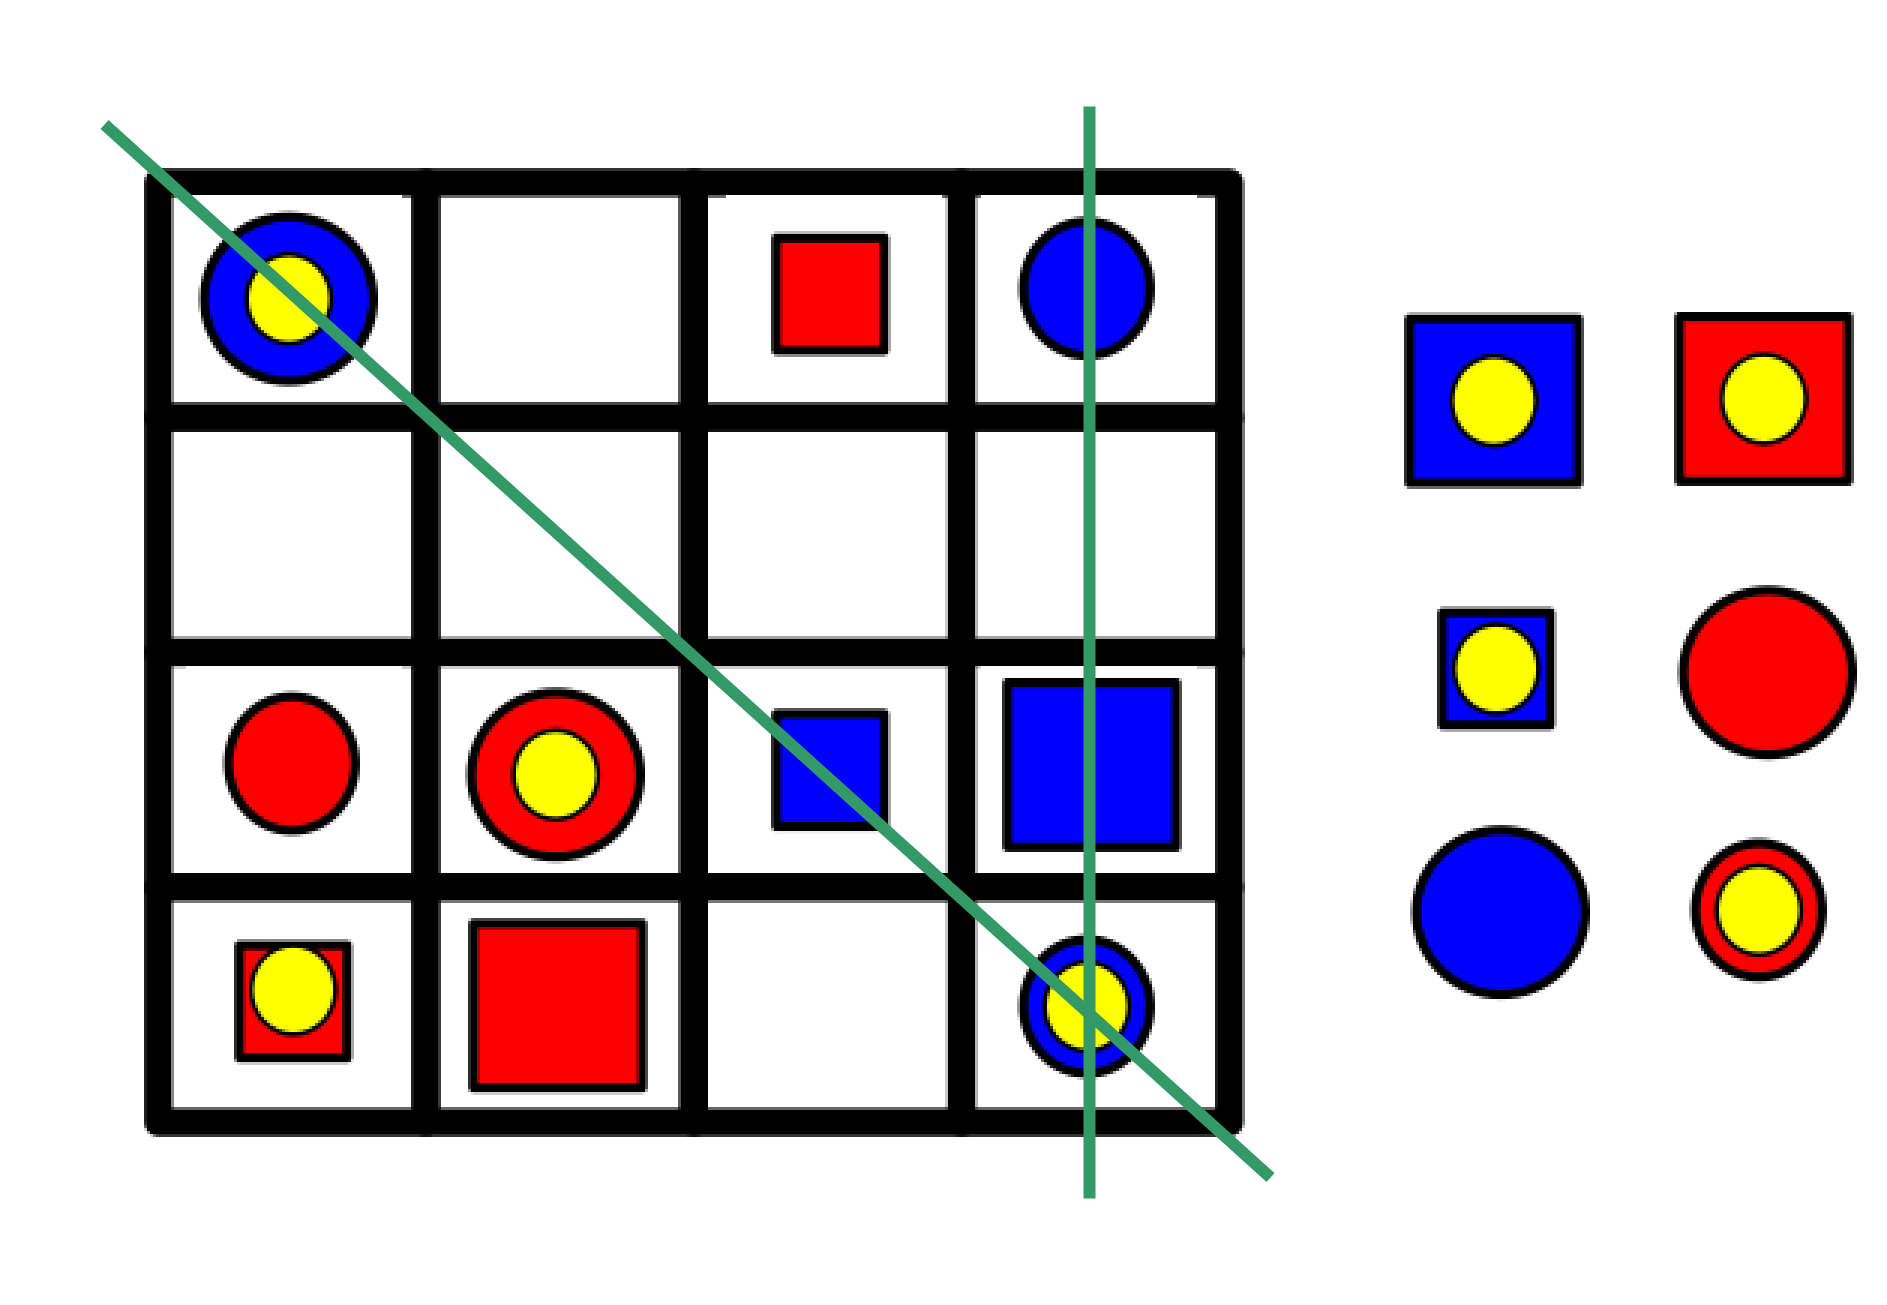
\includegraphics[height=0.2\textheight]{images/completingPiecesRelativeD}    
  \end{minipage}
  \caption{Comparison of two board states. The right board has a higher value $h$ returned by the evaluation function}
  \label{fig:relativeComparison}
\end{figure}
\subsubsection*{Conclusion}
To test the introduced heuristics we let them play against the trivial evaluation function which always returns 0. All of the heuristics described above were better then the trivial one which means that they indeed help to estimate a boards state and improve the performance of the MinMax Player.

A competition between the evaluation functions where all heuristics had to compete against each other has shown that the absolute completing pieces evaluation is the best. Therefore, the MinMax Player described in Chapter \ref{ch:evaluations} and \ref{ch:tournament} uses this evaluation function.
